\chapter{Component Failure Rate Data}
\label{appendix:componentFailureRate}
\graphicspath{ {./appendixC/Fig} }

This appendix contains failure rate data for selected electronic
components in support of Chapter 8. The information was abstracted from
the \ul{Military Handbook for Reliability Prediction}
{[}MIL-HDBK-217F{]} and contains information for devices that are
relevant to this book. The information is a close facsimile to
MIL-HDBK-217F, but in some instances comments are added to help
interpret the information. Furthermore, MIL-HDBK-217F tends to present
both empirical estimation formulas and tabular data computed from the
formulas. The tabular data is generally not included here for simplicity
of presentation, and is readily obtained from the formulas supplied.
Data is presented for the following devices:

\begin{itemize}
\item  Analog components: resistors and capacitors.
\item  Discrete semiconductors: diodes, bipolar transistors, and field effect  transistors.
\item  Microcircuits: gate/logic arrays and microprocessors.
\end{itemize}

\section{Environmental Use}
\label{section:environmental-use}

All of the devices presented in this appendix have an environmental
factor that is used to estimate the failure rate. The environmental
factors are based on the 14 categories in Table C.1.

\textbf{Table C.1}
\begin{table}
\caption{ Environmental symbols and descriptions taken directly
from MIL-HDBK-217F.}
\label{table:envSymbols}
\begin{tabular}{|l|m{10cm}|}
\hline
$G_{B}$ -- Ground, Benign & Nonmobile, temperature and
humidity controlled environments readily accessible to maintenance;
includes laboratory instruments and test equipment, medical electronic
equipment, business and scientific computer complexes, and missile and
support equipment in ground silos. \\ \hline
$G_{F}$ -- Ground, Fixed & Moderately controlled environments
such as installation in permanent racks with adequate cooling air and
possible installation in unheated buildings; includes permanent
installation of air traffic control radar and communication
facilities. \\ \hline
$G_{M}$ -- Ground, Mobile & Equipment installed in wheeled or
tracked vehicles and equipment manually transported; includes tactical
missile ground support equipment, mobile communication equipment,
tactical fire direction systems, handheld communications equipment,
laser designations and range finders. \\ \hline
$N_{S}$-- Naval, Sheltered & Includes sheltered or below
deck conditions on surface ships and equipment installed in
submarines. \\ \hline
$N_{U}$ -- Naval, Unsheltered & Unprotected surface shipborne
equipment exposed to weather conditions and equipment immersed in salt
water. Includes sonar equipment and equipment installed on hydrofoil
vessels. \\ \hline
$A_{IC}$-- Airborne, Inhabited Cargo & Typical conditions in
cargo compartments that can be occupied by an aircrew. Environment
extremes of pressure, temperature, shock, and vibration are minimal.
Examples include long mission aircraft such as the C130, C5, B52, and
C141. This category also applies to inhabited areas in lower performance
smaller aircraft such as the T38. \\ \hline
$A_{IF}$ -- Airborne, Inhabited Fighter & Same as 
$A_{IC}$ but installed on high performance aircraft such as
fighters and interceptors. Examples include the F15, F16, F111, F/A 18
and A10 aircraft. \\ \hline
$A_{UC}$ - Airborne, Uninhabited Cargo & Environmentally
uncontrolled areas that cannot be inhabited by crew during flight.
Environmental extremes of pressure, temperature, and shock may be
severe. Examples include uninhabited areas of long aircraft such as the
C130, C5, B52, and C141. This category also applies to uninhabited areas
in lower performance smaller aircraft such as the T38. \\
$A_{UF}$ - Airborne, Uninhabited Fighter & Same as
$A_{UC}$but installed on high performance aircraft such as
fighters and interceptors. Examples include the F15, F16, F111, and A10
aircraft. \\
$A_{RW}$-- Airborne, Rotary Winged & Equipment installed on
helicopters. Applies to both internally and externally mounted equipment
such as laser designators, fire control systems, and communications
equipment. \\
$S_{F}$ -- Space, Flight & Earth orbital. Approaches benign
ground conditions. Vehicle neither under powered flight nor in
atmospheric re-entry; includes satellites and shuttles. \\
$M_{F}$ -- Missile, Flight & Conditions related to powered
flight of air breathing missiles, cruise missiles, and missiles in
unpowered free flight. \\
$M_{L}$ -- Missile, Launch & Severe conditions related to
missile launch (air, ground, and sea), space vehicle boost into orbit,
and vehicle re-entry and landing by parachute. Also applies to solid
rocket motor propulsion powered flight, and torpedo and missile launch
from submarines. \\
$C_{L}$ -- Cannon, Launch & Extremely severe conditions
related to cannon launching of 155 mm and 5 inch guided projectiles.
Conditions apply to the projectile from launch to target impact. \\
\end{tabular}
\end{table}

\section{Analog Components: Resistors and Capacitors}
\label{section:analog-components-resistors-and-capacitors}

This section contains failure rate data for resistors and capacitors.

\subsection{Resistors: Fixed Composition, Fixed Film, and Wirewound}
\label{section:resistors-fixed-composition-fixed-film-and-wirewound}

The failure rate is given by the following relationship

$$\lambda = \lambda_{b} \pi_{R} \pi_{Q} \pi_{E} \frac{failures}{10^{6} hours}$$.




\begin{table}
\caption{$\lambda_{b} = $ \textbf{Base Failure Rate}}
\label{table:baseFailureRate}
\begin{tabular}{|l|m{10cm}|} \hline
\rowcolor{Gray}
\textbf{Resistor Type} &
$\lambda_b$ 
$(T = ambient temperatire in ^\circ C, S = \frac{operating power}{device power rating})$ \\ \hline
Fixed Composition & 
$\lambda_b = 4.5x10^{-9} exp [12(\frac{T+273}{343})] exp[\frac{S}{0.6}(\frac{T+273}{273})]$ \\ \hline
Fixed Film &
$\lambda_b = 3.25x10^{-4} exp [12(\frac{T+273}{343})^3] exp[S(\frac{T+273}{273})]$ \\ \hline
Wirewound &
$\lambda_b = 0.0031 exp [12(\frac{T+273}{343})^{10}] exp\{[\frac{S}{0.6}(\frac{T+273}{273})]^{1.5}\}$ \\ \hline
\end{tabular}
\end{table}




\begin{table}
\caption{\textbf{Resistance Factor -} $\pi_{R}$}
\label{table:resistanceFactor}
\begin{tabular}{|c|c|c|c|} \hline
\rowcolor{Gray}
\multicolumn{2}{|l|}{\textbf{Fixed Composition or Fixed Film Resistors}} &  \multicolumn{2}{|l|}{\textbf{Wirewound Resistors}} \\ \hline
\textbf{Resistance Range} & $\pi_{R}$ & \textbf{Resistance Range} & $\pi_{R}$ \\ \hline
$ \leq 100k\Omega$                            & 1.0 & $ \leq 10k\Omega$                                     & 1.0 \\ \hline
$ 100k\Omega$ to $\leq 1M\omega$ & 1.1 & $ 10k\Omega$ to $\leq 100k\omega$  & 1.7 \\ \hline
$ 1M\Omega$ to $\leq 10M\omega$  & 1.6 & $ 100k\Omega$ to $\leq 1M\omega$  & 3.0 \\ \hline
$ > 10M\Omega$                                 & 2.5 & $ > 1M\Omega$                                     & 5.0 \\ \hline
\end{tabular}
\end{table}



\begin{table}
\caption{\textbf{Quality Factor -} $\pi_{Q}$}
\label{table:qualityFactor}
\begin{tabular}{|c|c|} \hline
\textbf{Quality} & $\pi_{Q}$ \\ \hline
S & 0.03 \\ \hline
R & 0.1 \\ \hline
P & 0.3 \\ \hline
M & 1.0 \\ \hline
MIL-R & 5.0 \\ \hline
Lower & 15 \\ \hline
\end{tabular}
\end{table}


\begin{table}
\caption{\textbf{Environmental factor -} $\pi_{E}$}
\label{table:environmentalFactor}
\begin{tabular}{|c|c|c|c|} \hline
\textbf{Environment} & $\pi_{E}$ \textbf{Fixed Composition} & $\pi_{E}$ \textbf{Fixed Film} & $\pi_{E}$ \textbf{Wirewound} \\ \hline
$G_{B}$ & 1 & 1 & 1 \\  \hline
$G_{F}$ & 3 & 2 & 2 \\ \hline
$G_{M}$ & 8 & 8 & 11 \\ \hline
$N_{S}$ & 5 & 4 & 5 \\ \hline
$N_{U}$ & 13 & 14 & 18 \\ \hline
$A_{IC}$ & 4 & 4 & 15 \\ \hline
$A_{IF}$ & 5 & 8 & 18 \\ \hline
$A_{UC}$ & 7 & 10 & 28 \\ \hline
$A_{UF}$ & 11 & 18 & 35 \\ \hline
$A_{RW}$ & 19 & 19 & 27 \\ \hline
$S_{F}$ & 0.50 & 0.20 & 0.80 \\ \hline
$M_{F}$ & 11 & 10 & 14 \\ \hline
$M_{L}$ & 27 & 28 & 38 \\ \hline
$C_{L}$ & 490 & 510 & 610 \\ \hline
\end{tabular}
\end{table}

\subsection{Capacitors: Fixed, Ceramic, and General Purpose}
\label{subsection:capacitors-fixed-ceramic-and-general-purpose}

The failure rate is given by the following relationship
$$\lambda = \lambda{b} \Pi_{CV} \Pi_{Q} \Pi_{E} \frac{failures}{10^{6} hours}$$

For all factors $T$ = ambient temperature ($^\circ$C) and 
$S=\frac{operating voltage}{rated voltage}$, where the
operating voltage is the sum of the DC and peak AC voltage.

\begin{table}
\caption{\textbf{Base Failure Rate -} $\lambda_{b}$}
\label{table:baseFailureRate}
\begin{tabular}{l}
$\lambda_b = 0.0003 [\frac{S}{0.3}^{3}] exp [\frac{T+273}{358}]$ for T=85$^{circ}$C max rated \\ 
$\lambda_b = 0.0003 [\frac{S}{0.3}^{3}] exp [\frac{T+273}{398}]$ for T=125$^{circ}$C max rated \\ 
$\lambda_b = 0.0003 [\frac{S}{0.3}^{3}] exp [\frac{T+273}{423}]$ for T=150$^{circ}$C max rated \\ 
\end{tabular}
\end{table}


\begin{table}
\caption{\textbf{Capacitance Factor -} $\Pi_{CV}$}
\label{table:capacitanceFactor}
\begin{tabular}{|l|m{10cm}|} \hline
\textbf{Quality} & $\Pi_{Q}$ \\ \hline
S & 0.030 \\ \hline
R & 0.10 \\ \hline
P & 0.30 \\ \hline
M & 1.0 \\ \hline
L & 3.0 \\ \hline
MIL & 3.0 \\ \hline
Lower & 10 \\ \hline
\end{tabular}
\end{table}

\begin{table}
\caption{\textbf{Environmental Factor -} $\Pi_{E}$}
\label{table:capacitanceFactor}
\begin{tabular}{|l|m{10cm}|} \hline
\textbf{Environment} & $\Pi_{E}$ \\ \hline
$G_{B}$ & 1 \\ \hline
$G_{F}$ & 2 \\ \hline
$G_{M}$ & 9 \\ \hline
$N_{S}$ & 5 \\ \hline
$N_{U}$ & 15 \\ \hline
$A_{IC}$ & 4 \\ \hline
$A_{IF}$ & 4 \\ \hline
$A_{UC}$ & 8 \\ \hline
$A_{UF}$ & 12 \\ \hline
$A_{RW}$ & 20 \\ \hline
$S_{F}$ & 0.40 \\ \hline
$M_{F}$ & 13 \\ \hline
$M_{L}$ & 34 \\ \hline
$C_{L}$ & 610 \\ \hline
\end{tabular}
\end{table}


\section{Microelectronic Devices}
\label{section:microelectronic-devices}

For all microelectronic devices it is necessary to compute the junction
temperature ($T_{j}$) of the silicon in order to determine the temperature 
factor. The junction temperature is determined as follows:

$$T_{j} = T_{A} \theta_{jA} P_{D}$$
$$T_A = $$ ambient temperature
$$\theta_{jA} = $$junction to ambient thermal resistance (obtained from manufacture data sheet.)
$$P_{D} = $$power dissipated inm the device

\textbf{Author's Note:} The equations above are slightly different than
those found in MIL-HDBK-217F. The junction to ambient thermal resistance
is used here, instead of junction to case as in the original. In
addition, the ambient temperature is used in place of the case
temperature. This is more general and is consistent with the
presentation in Chapter~\ref{chapter:systemReliability}. The junction to case 
resistance could be used, along with the case temperature. See 
Section~\ref{section:reliability-prediction} for more detailed
coverage of this thermal model.

The part quality descriptors in Table~\ref{table:partsQualityDescriptors} are used to find the quality
factors.

\begin{table}
\caption{Part quality descriptors for microelectronic devices.}
\label{table:partsQualityDescriptors}
\begin{tabular}{|l|m{10cm}|} \hline
\textbf{JANTXV} & 
Full device testing as specified by the MIL-S-19500 specification,
including Screening and Groups A, B, and C. \\ \hline
\textbf{JANTX} & Identical to JANTXV, except does not include the 100\%
precap visual inspection contained in Screening. \\ \hline
\textbf{JAN} & Testing as defined by MIL-S-19500, including Groups A, B,
and C, but not including Screening. \\ \hline
\textbf{Lower} & All hermetically packaged devices. \\ \hline
\textbf{Plastic} & All devices encapsulated with organic materials. \\ \hline
\end{tabular}
\end{table}


\subsection{Diodes: Low Frequency}
\label{subsection:diodes-low-frequency}

The failure rate is given by the following relationship

$$\lambda = \lambda{b} \Pi_{R} \Pi_{Q} \Pi_{E} \frac{failures}{10^{6} hours}$$

\begin{table}
\caption{\textbf{Base Failure Rate -} $\lambda_{b}$}
\label{table:baseFailRateDiodeLow}
\begin{tabular}{|l|m{10cm}|} \hline
\textbf{Diode Type/Application} & $\lambda_{b}$ \\ \hline
General purpose analog & 0.0038 \\ \hline
Switching & 0.0010 \\ \hline
Power rectifier, fast recovery & 0.069 \\ \hline
Power rectifier, Schottky power diode & 0.0030 \\ \hline
Power rectifier with high voltage stacks & 0.0050/Junction \\ \hline
Transient suppressor/varistor & 0.0013 \\ \hline
Current regulator & 0.0034 \\ \hline
Voltage regulator and voltage reference (avalanche and zener) &
0.0020 \\ \hline
\end{tabular}
\end{table}

\textbf{Temperature Factor -} $\Pi_{T}$

For general purpose analog, switching, fast recovery, power rectifier,
and transient suppressor applications

$$\Pi_{T} = exp[-3091(\frac{1}{T_{j} + 273} - \frac{1}{298})].$$

For voltage regulator, voltage reference, and current regulator
applications

$$\Pi_{T} = exp[-1925(\frac{1}{T_{j} + 273} - \frac{1}{298})].$$


\begin{table}
\caption{\textbf{Electrical Stress Factor -} $\Pi_{S}$}
\label{table:electicalStressFactor}
\begin{tabular}{|l|l|}
$\Pi_s = 0.054$ 		& $V_{S} \leq 0.3$ \\ 
$\Pi_s = V^{2.43}_{S}$ & $0.3 < V_{S} \leq 1$ \\
\end{tabular}
\end{table}

\begin{table}
\caption{\textbf{Quality Factor -} $\Pi_{Q}$}
\label{table:qualityFactorDiode}
\begin{tabular}{|l|m{10cm}|} \hline
\textbf{Quality} & $\Pi_{Q}$ \\ \hline
JANTXV & 0.7 \\ \hline
JANTX & 1.0 \\ \hline
JAN & 2.4 \\ \hline
Lower & 5.5 \\ \hline
Plastic & 8.0 \\ \hline
\end{tabular}
\end{table}


\begin{table}
\caption{\textbf{Contact Construction Factor -} $\Pi_{C}$}
\label{table:<context>}
\begin{tabular}{|l|m{10cm}|} \hline
\textbf{Contact Construction} & $\Pi_{C}$ \\ \hline
Metallurgically bonded & 1.0 \\ \hline
Non-metallurgically bonded and spring loaded contacts & 2.0 \\ \hline\end{tabular}
\end{table}


\begin{table}
\caption{
\textbf{Environmental Factor -} $\Pi_{E}$}
\label{table:enviroFactorDiode}
\begin{tabular}{|l|m{10cm}|} \hline
\textbf{Environment} & $\Pi_{E}$ \\ \hline
$G_{B}$ & 1 \\ \hline
$G_{F}$ & 6 \\ \hline
$G_{M}$ & 9 \\ \hline
$N_{S}$ & 9 \\ \hline
$N_{U}$ & 19 \\ \hline
$A_{IC}$ & 13 \\ \hline
$A_{IF}$ & 29 \\ \hline
$A_{UC}$ & 20 \\ \hline
$A_{UF}$ & 43 \\ \hline
$A_{RW}$ & 24 \\ \hline
$S_{F}$ & 0.50 \\ \hline
$M_{F}$ & 14 \\ \hline
$M_{L}$ & 32 \\ \hline
$C_{L}$ & 320 \\ \hline
\end{tabular}
\end{table}



\subsection{Diodes: High Frequency (microwave, RF)}
\label{subsection:diodes-high-frequency-microwave-rf}

The failure rate is given by the following relationship

$$\lambda = \lambda{b} \Pi_{R} \Pi_{Q} \Pi_{E} \frac{failures}{10^{6} hours}$$


\begin{table}
\caption{\textbf{Base Failure Rate} - $\lambda_{b}$}
\label{table:baseFailureRateDiodeHigh}
\begin{tabular}{|l|m{10cm}|} \hline
\textbf{Diode Type} & $\lambda_{b}$ \\ \hline
Si IMPATT $\leq 35$GHz) & 0.22 \\ \hline
Gunn/Bulk Effect & 0.18 \\ \hline
Tunnel and Back & 0.0023 \\ \hline
PIN & 0.0081 \\ \hline
Schottky Barrier & 0.027 \\ \hline
Varactor and Step Recovery & 0.0025 \\ \hline
\end{tabular}
\end{table}

\begin{table}
\caption{\textbf{Application Factor -} $\Pi_{A}$}
\label{table:applicationFactorHigh}
\begin{tabular}{|l|m{10cm}|} \hline
\textbf{Application} & $\Pi_{A}$ \\ \hline
Varactor, voltage control & 0.50 \\ \hline
Varactor, multiplier & 2.5 \\ \hline
All other diodes & 1.0 \\ \hline
\end{tabular}
\end{table}

\begin{table}
\caption{\textbf{Quality Factor -} $\Pi_{Q}$}
\label{table:applicationFactorHigh}
\begin{tabular}{|c|c|c|} \hline
\textbf{Quality} & \textbf{Not Shottky} & \textbf{Shottky} \\ \hline
JANTXV & 0.5 & 0.5 \\ \hline
JANTX & 1.0 & 1.0 \\ \hline
JAN & 5.0 & 1.8 \\ \hline
Lower & 25.0 & 2.5 \\ \hline
Plastic & 50.0 & - \\ \hline
\end{tabular}
\end{table}


\begin{table}
\caption{\textbf{Temperature Factor -} $\Pi_{T}$  }
\label{table:temperatureFactorHigh}
\begin{tabular}{l l}  
All types except IMPATT & and for IMPATT \\
$\Pi_{T} = exp[-2100(\frac{1}{T_{J}} - \frac{1}{298})]$ & 
$\Pi_{T} = exp[-5260(\frac{1}{T_{J}} - \frac{1}{298})]$ \\ 
\end{tabular}
\end{table}





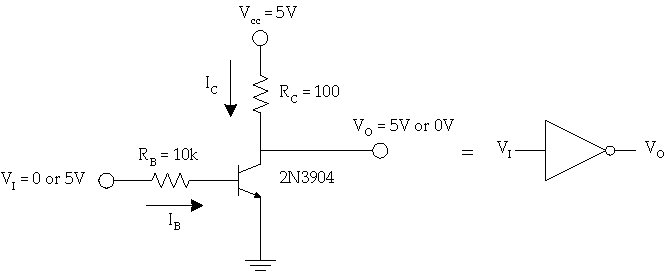
\includegraphics{Fig/media/image63.wmf}.

\textbf{Power Rating Factor -} 
\includegraphics{Fig/media/image64.wmf}


\includegraphics{Fig/media/image65.wmf}

\textbf{Environmental Factor -} 
\includegraphics{Fig/media/image66.wmf}

\begin{longtable}[]{@{}
  >{\raggedright\arraybackslash}p{(\columnwidth - 2\tabcolsep) * \real{0.6675}}
  >{\raggedright\arraybackslash}p{(\columnwidth - 2\tabcolsep) * \real{0.3325}}@{}}
\toprule\noalign{}
\begin{minipage}[b]{\linewidth}\raggedright
\textbf{Environment}
\end{minipage} & \begin{minipage}[b]{\linewidth}\raggedright
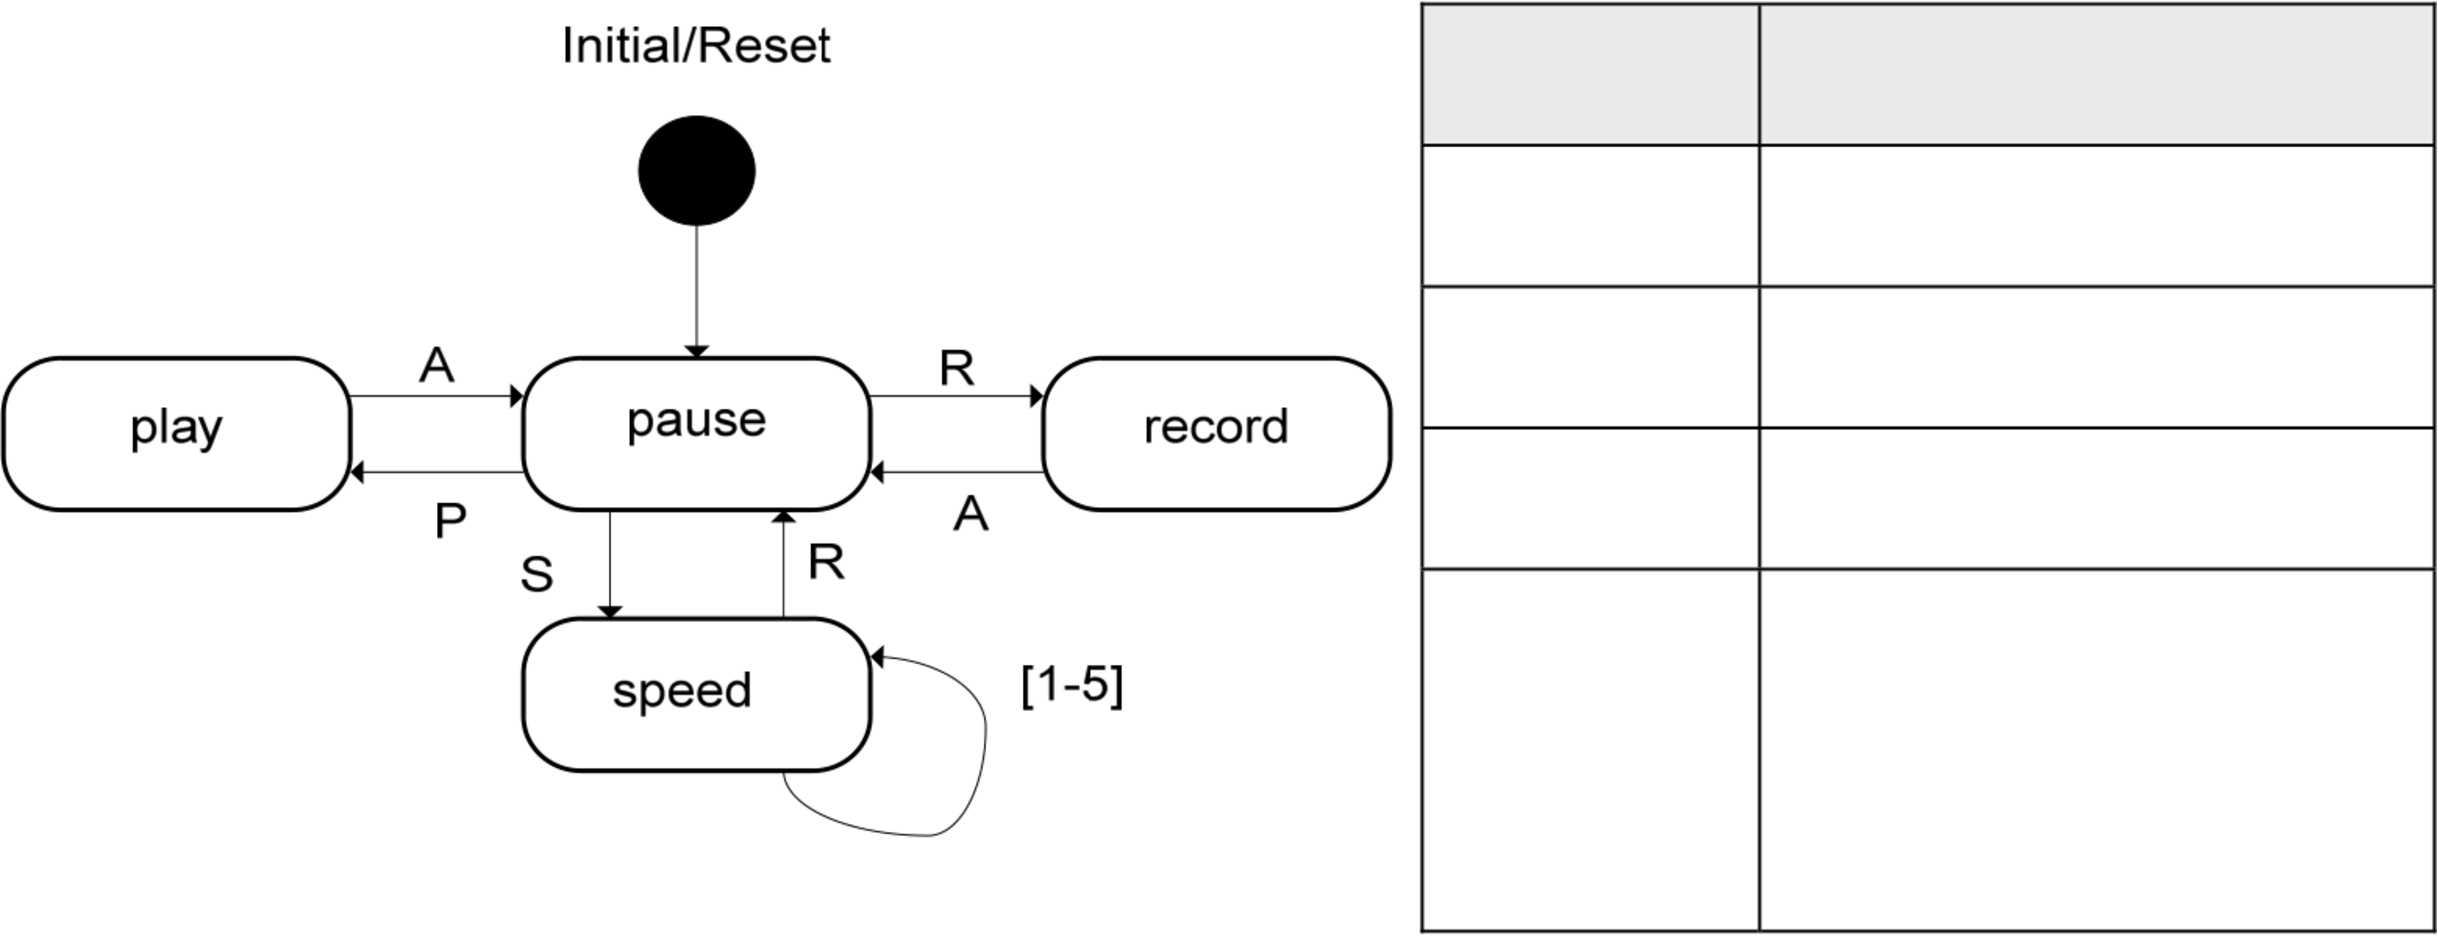
\includegraphics{Fig/media/image67.wmf}
\end{minipage} \\
\midrule\noalign{}
\endhead
\bottomrule\noalign{}
\endlastfoot
G\textsubscript{B} & 1 \\
G\textsubscript{F} & 2 \\
G\textsubscript{M} & 5 \\
N\textsubscript{S} & 4 \\
N\textsubscript{U} & 11 \\
A\textsubscript{IC} & 4 \\
A\textsubscript{IF} & 5 \\
A\textsubscript{UC} & 7 \\
A\textsubscript{UF} & 12 \\
A\textsubscript{RW} & 16 \\
S\textsubscript{F} & 0.5 \\
M\textsubscript{F} & 9 \\
M\textsubscript{L} & 24 \\
C\textsubscript{L} & 250 \\
\end{longtable}
\end{minipage} \\
\midrule\noalign{}
\endhead
\bottomrule\noalign{}
\endlastfoot
\end{longtable}

\subsubsection{\texorpdfstring{\hfill\break
Transistors: Bipolar Junction, Low Frequency (≤
200MHz)}{ Transistors: Bipolar Junction, Low Frequency (≤ 200MHz)}}\label{transistors-bipolar-junction-low-frequency-200mhz}

The failure rate is given by the following relationship


\includegraphics{Fig/media/image68.wmf}.

\begin{longtable}[]{@{}
  >{\raggedright\arraybackslash}p{(\columnwidth - 4\tabcolsep) * \real{0.5301}}
  >{\raggedright\arraybackslash}p{(\columnwidth - 4\tabcolsep) * \real{0.0689}}
  >{\raggedright\arraybackslash}p{(\columnwidth - 4\tabcolsep) * \real{0.4010}}@{}}
\toprule\noalign{}
\begin{minipage}[b]{\linewidth}\raggedright
\textbf{Base Failure Rate -} 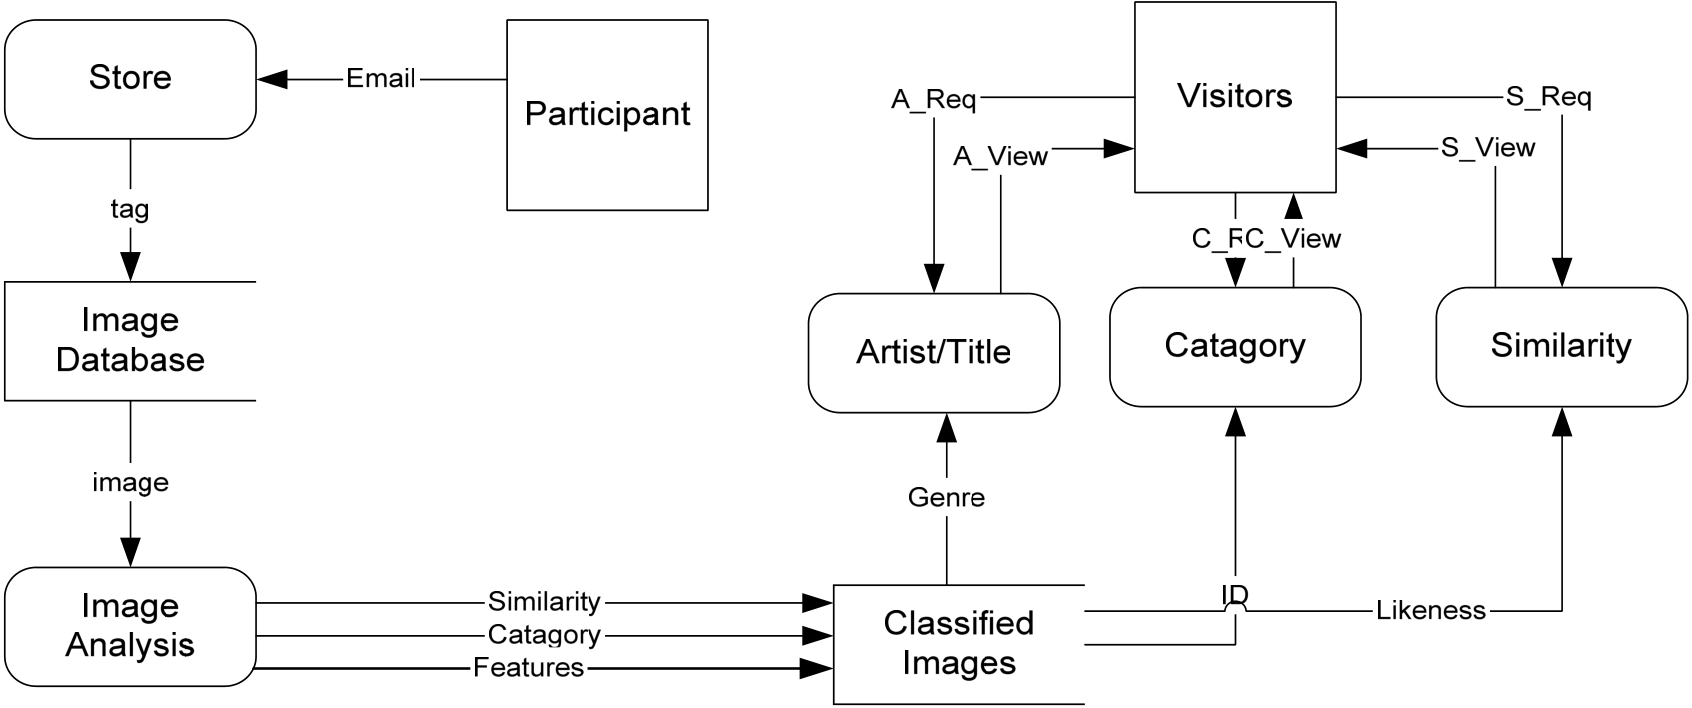
\includegraphics{Fig/media/image69.wmf}

\begin{longtable}[]{@{}
  >{\raggedright\arraybackslash}p{(\columnwidth - 2\tabcolsep) * \real{0.6164}}
  >{\raggedright\arraybackslash}p{(\columnwidth - 2\tabcolsep) * \real{0.3836}}@{}}
\toprule\noalign{}
\begin{minipage}[b]{\linewidth}\raggedright
\textbf{Type}
\end{minipage} & \begin{minipage}[b]{\linewidth}\raggedright
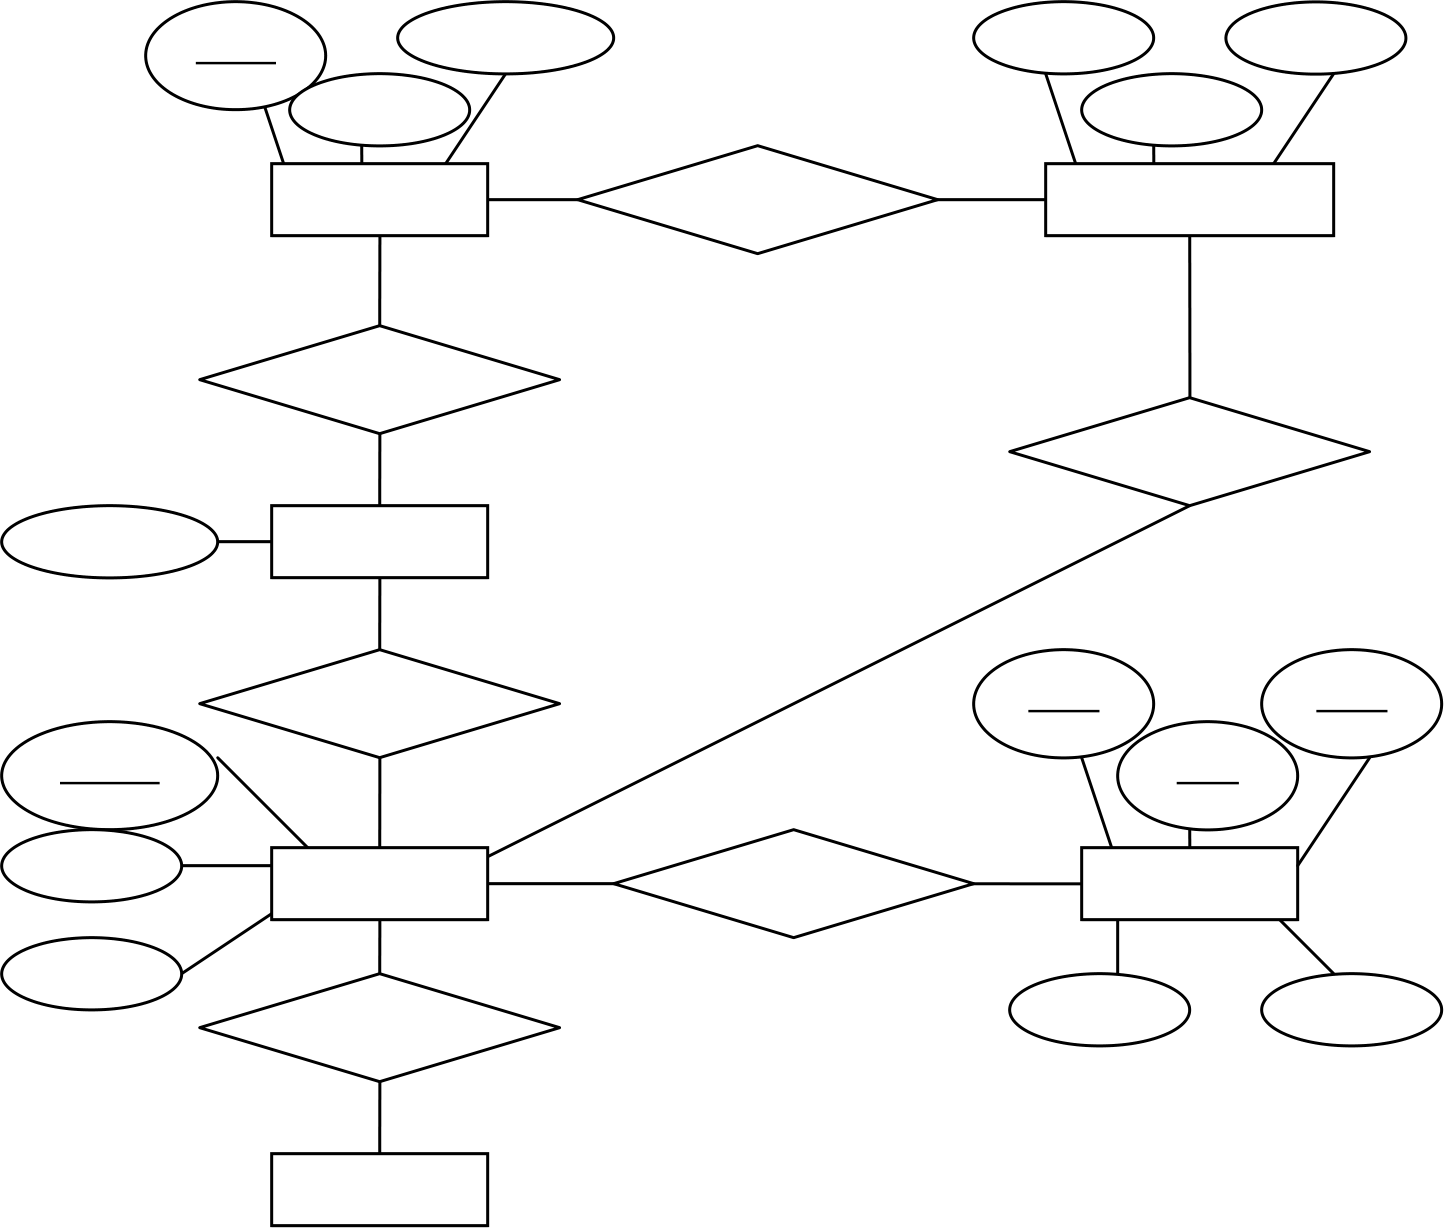
\includegraphics{Fig/media/image70.wmf}
\end{minipage} \\
\midrule\noalign{}
\endhead
\bottomrule\noalign{}
\endlastfoot
NPN or PNP & 0.00074 \\
\end{longtable}

\textbf{Temperature Factor -} 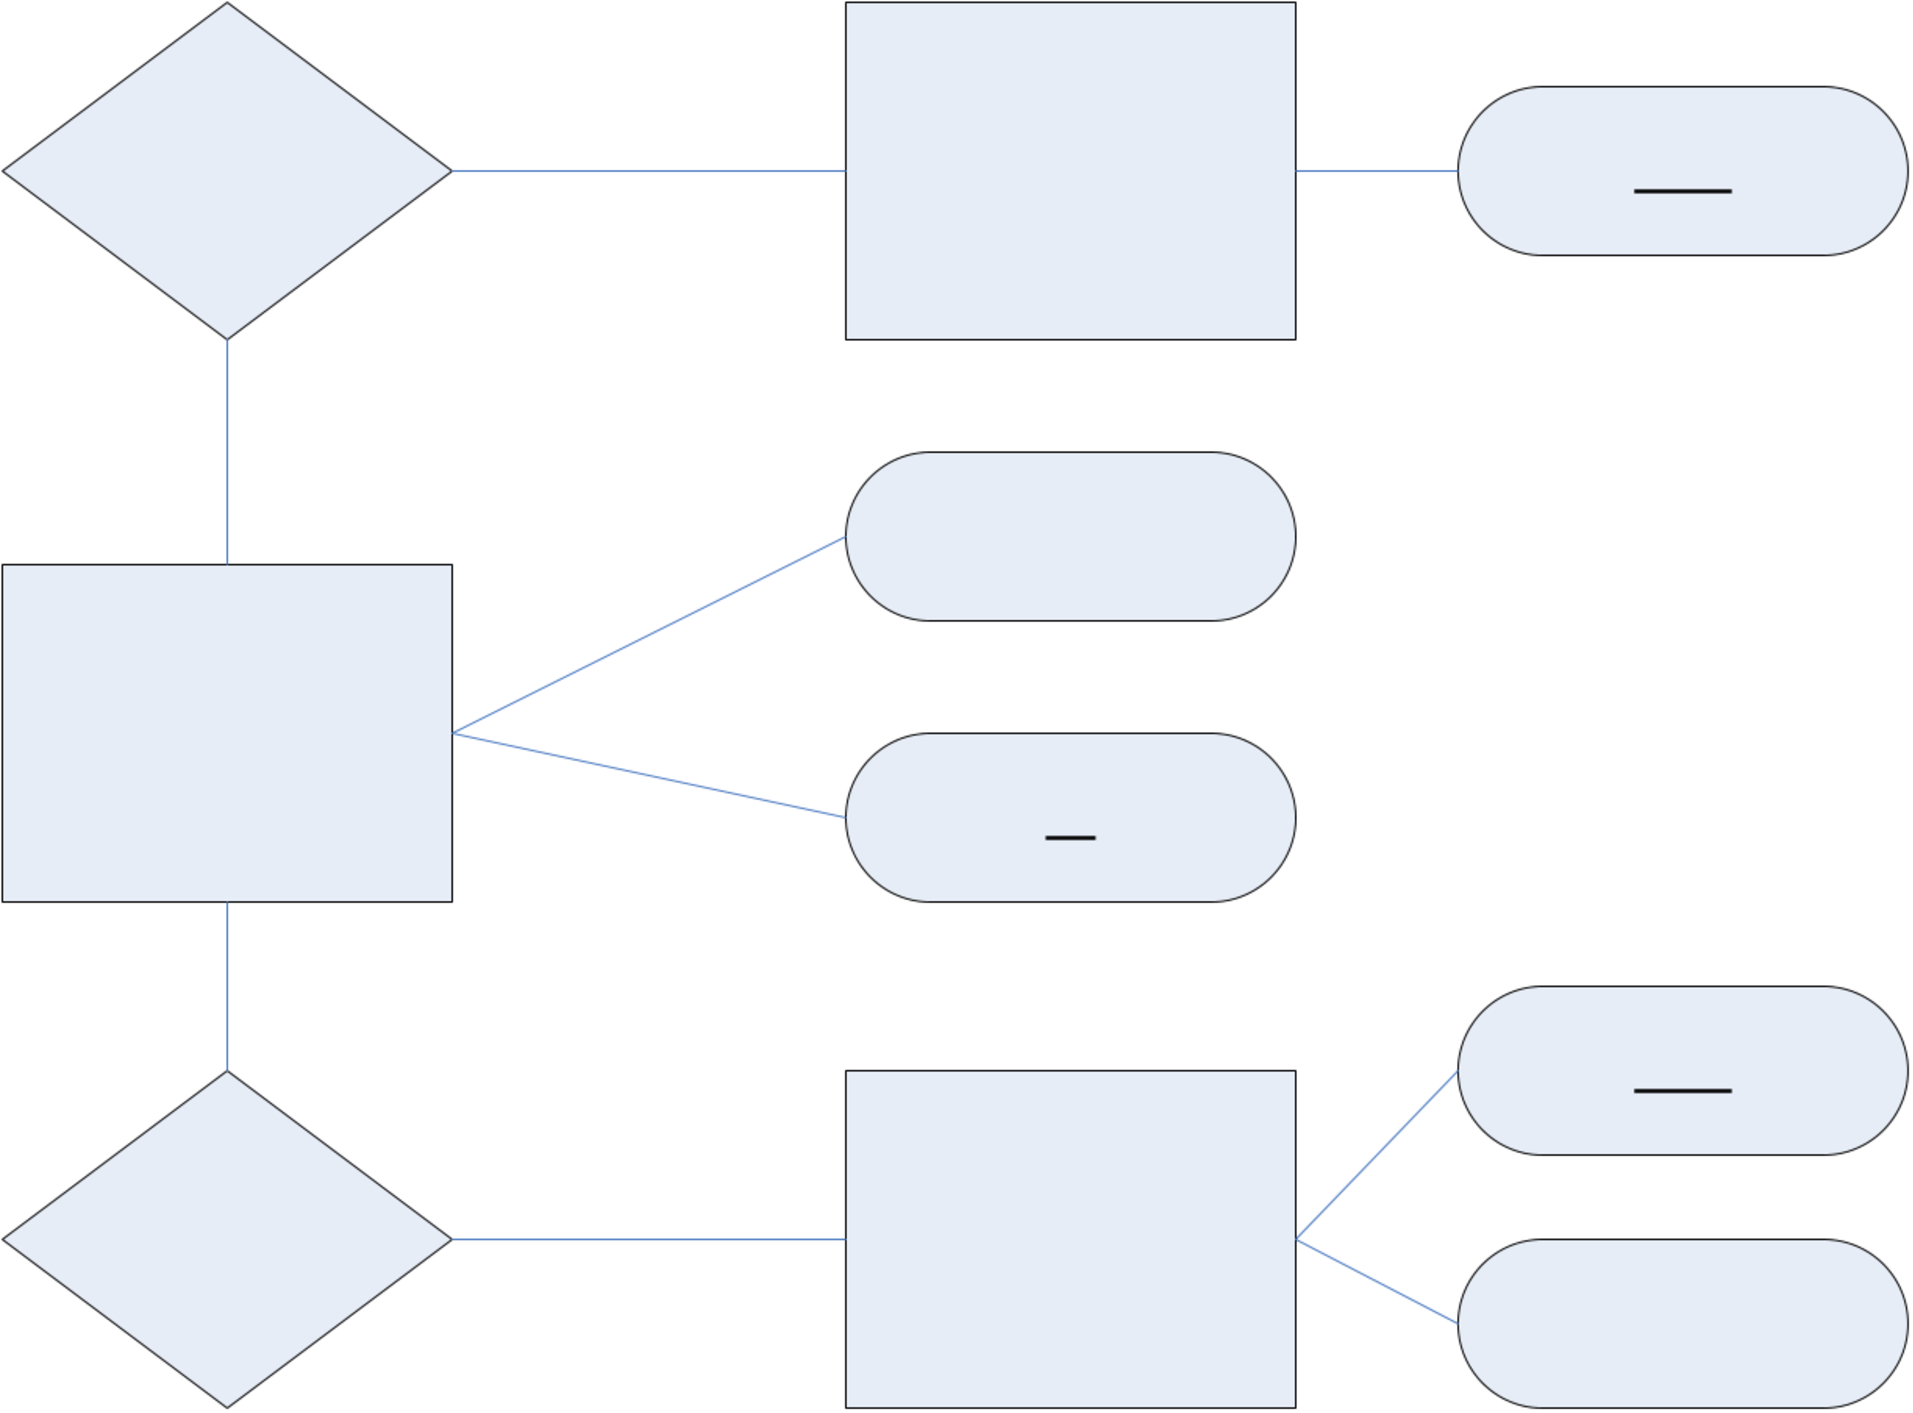
\includegraphics{Fig/media/image71.wmf}

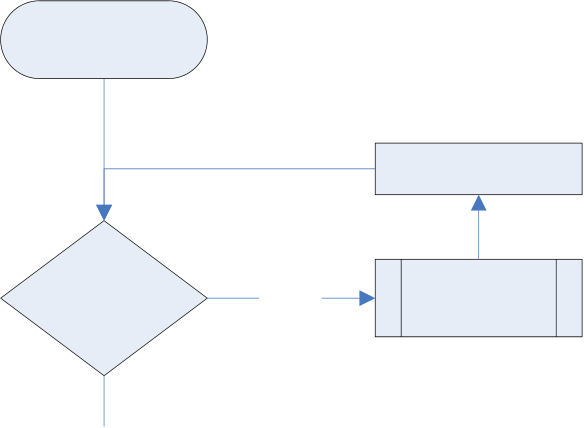
\includegraphics{Fig/media/image72.wmf}

\textbf{Application Factor -} 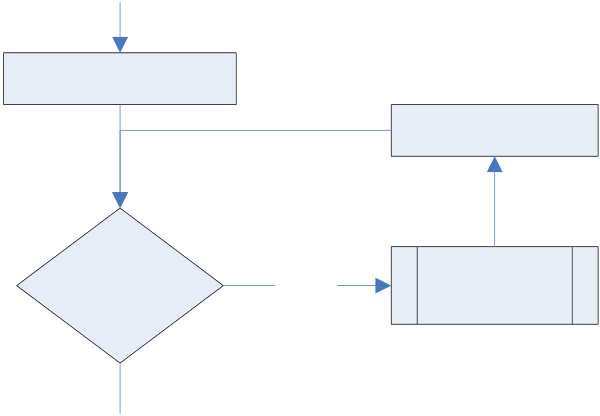
\includegraphics{Fig/media/image73.wmf}

\begin{longtable}[]{@{}
  >{\raggedright\arraybackslash}p{(\columnwidth - 2\tabcolsep) * \real{0.7360}}
  >{\raggedright\arraybackslash}p{(\columnwidth - 2\tabcolsep) * \real{0.2640}}@{}}
\toprule\noalign{}
\begin{minipage}[b]{\linewidth}\raggedright
\textbf{Application}
\end{minipage} & \begin{minipage}[b]{\linewidth}\raggedright
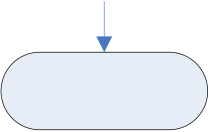
\includegraphics{Fig/media/image74.wmf}
\end{minipage} \\
\midrule\noalign{}
\endhead
\bottomrule\noalign{}
\endlastfoot
Linear Amplification & 1.50 \\
Switching & 0.70 \\
\end{longtable}

\textbf{Power Rating Factor -} 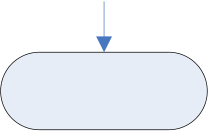
\includegraphics{Fig/media/image75.wmf}

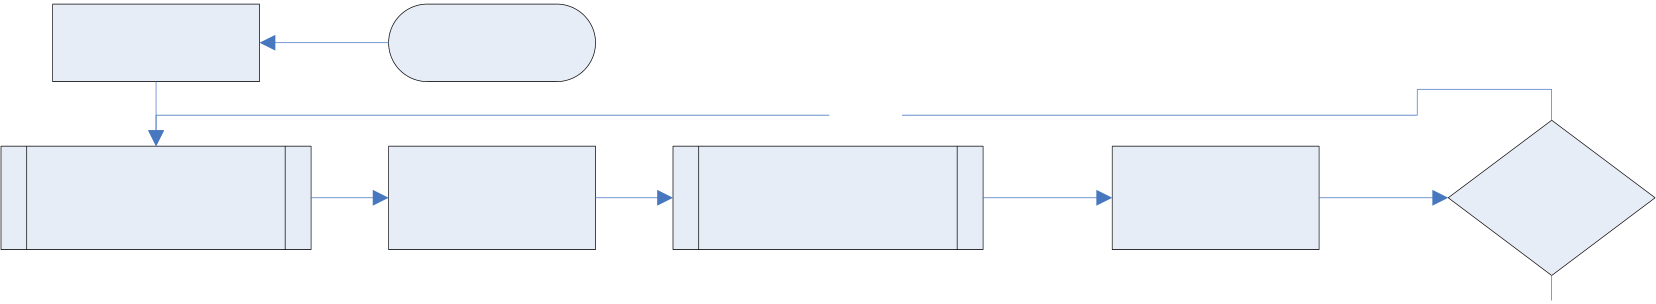
\includegraphics{Fig/media/image76.wmf}

\textbf{Voltage Stress Factor -} 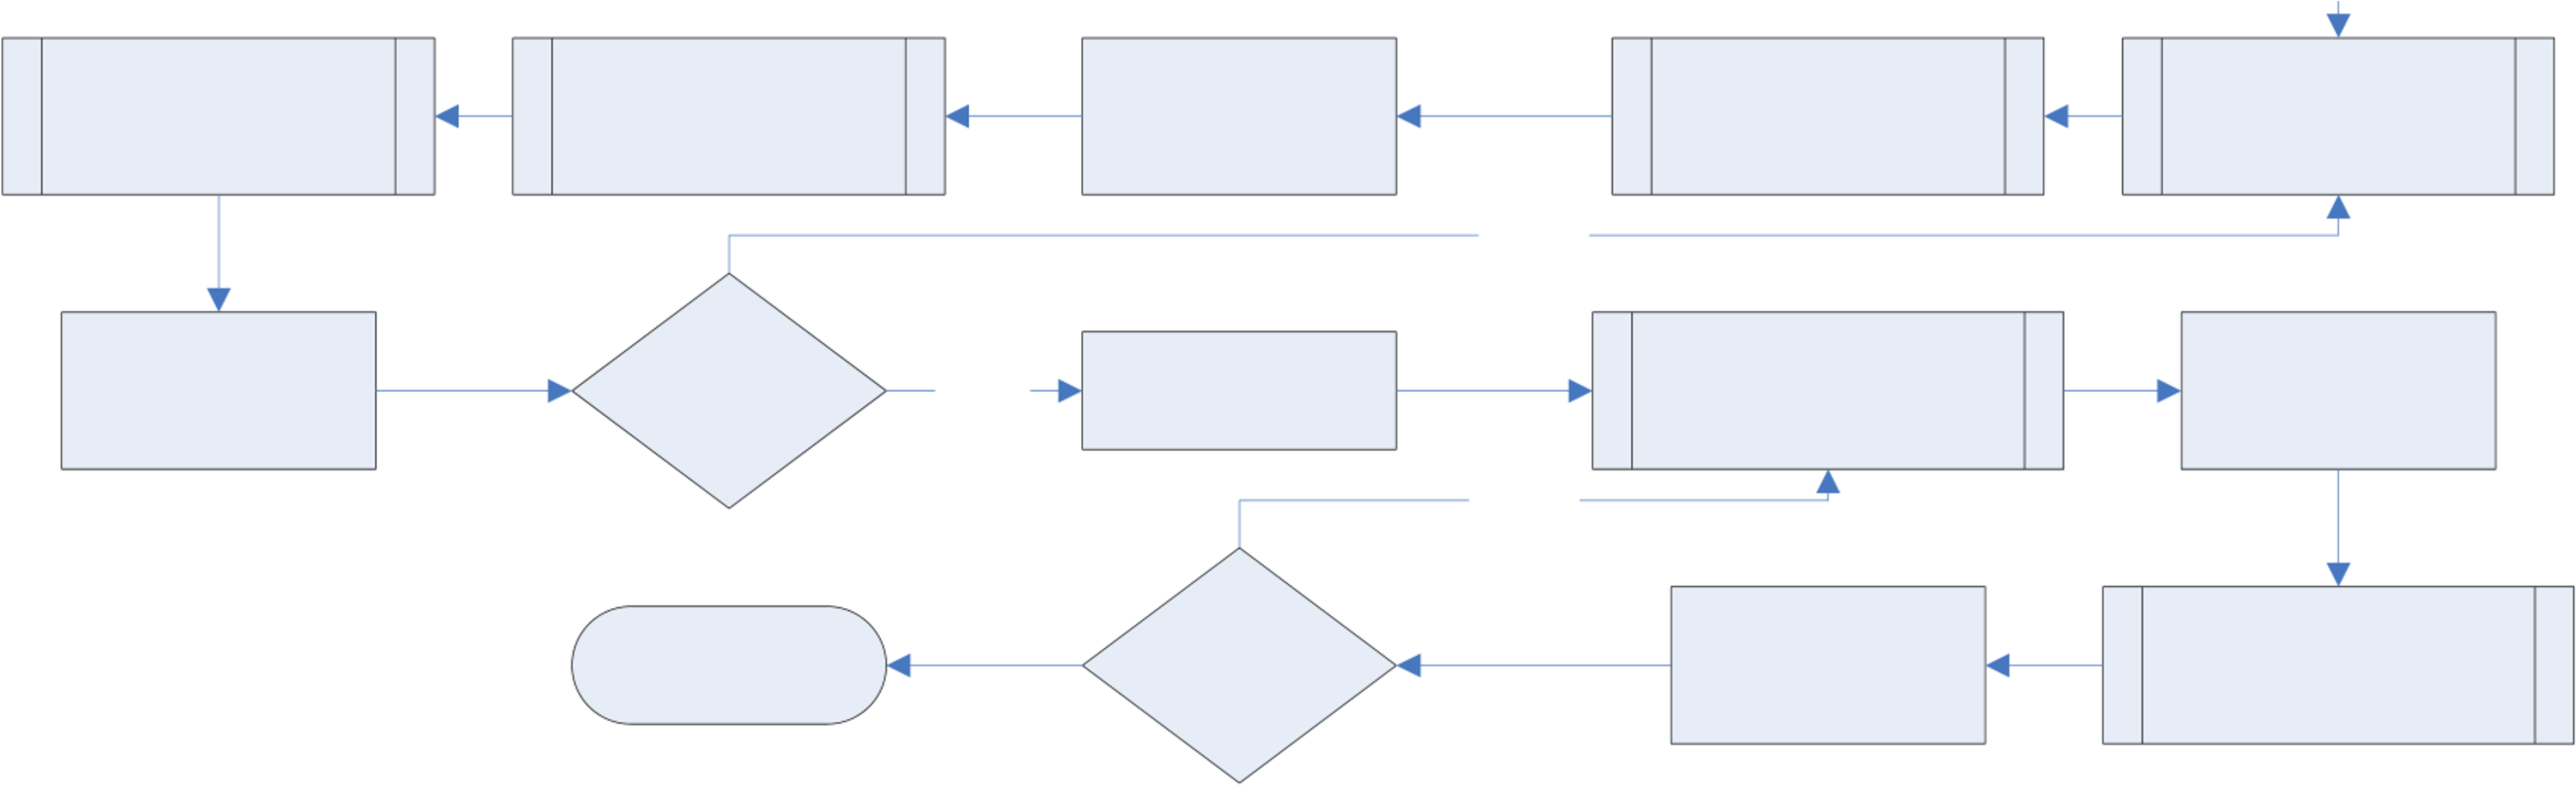
\includegraphics{Fig/media/image77.wmf}

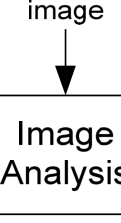
\includegraphics{Fig/media/image78.wmf}
\end{minipage} & \begin{minipage}[b]{\linewidth}\raggedright
\end{minipage} & \begin{minipage}[b]{\linewidth}\raggedright
\textbf{Part Quality Factor -} 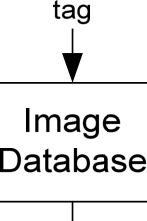
\includegraphics{Fig/media/image79.wmf}

\begin{longtable}[]{@{}
  >{\raggedright\arraybackslash}p{(\columnwidth - 2\tabcolsep) * \real{0.6364}}
  >{\raggedright\arraybackslash}p{(\columnwidth - 2\tabcolsep) * \real{0.3636}}@{}}
\toprule\noalign{}
\begin{minipage}[b]{\linewidth}\raggedright
\textbf{Quality}
\end{minipage} & \begin{minipage}[b]{\linewidth}\raggedright

\includegraphics{Fig/media/image80.wmf}
\end{minipage} \\
\midrule\noalign{}
\endhead
\bottomrule\noalign{}
\endlastfoot
JANTXV & 0.7 \\
JANTX & 1.0 \\
JAN & 2.4 \\
Lower & 5.5 \\
Plastic & 8.0 \\
\end{longtable}

\textbf{Environmental Factor -} 
\includegraphics{Fig/media/image81.wmf}

\begin{longtable}[]{@{}
  >{\raggedright\arraybackslash}p{(\columnwidth - 2\tabcolsep) * \real{0.7079}}
  >{\raggedright\arraybackslash}p{(\columnwidth - 2\tabcolsep) * \real{0.2921}}@{}}
\toprule\noalign{}
\begin{minipage}[b]{\linewidth}\raggedright
\textbf{Environment}
\end{minipage} & \begin{minipage}[b]{\linewidth}\raggedright
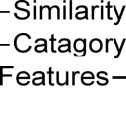
\includegraphics{Fig/media/image82.wmf}
\end{minipage} \\
\midrule\noalign{}
\endhead
\bottomrule\noalign{}
\endlastfoot
G\textsubscript{B} & 1 \\
G\textsubscript{F} & 6 \\
G\textsubscript{M} & 9 \\
N\textsubscript{S} & 9 \\
N\textsubscript{U} & 19 \\
A\textsubscript{IC} & 13 \\
A\textsubscript{IF} & 29 \\
A\textsubscript{UC} & 20 \\
A\textsubscript{UF} & 43 \\
A\textsubscript{RW} & 24 \\
S\textsubscript{F} & 0.50 \\
M\textsubscript{F} & 14 \\
M\textsubscript{L} & 32 \\
C\textsubscript{L} & 320 \\
\end{longtable}
\end{minipage} \\
\midrule\noalign{}
\endhead
\bottomrule\noalign{}
\endlastfoot
\end{longtable}

\subsubsection{\texorpdfstring{\hfill\break
Transistors: Bipolar Junction, High Frequency (\textgreater{} 200MHz),
Low Noise (Power ≤
1W)}{ Transistors: Bipolar Junction, High Frequency (\textgreater{} 200MHz), Low Noise (Power ≤ 1W)}}\label{transistors-bipolar-junction-high-frequency-200mhz-low-noise-power-1w}

The failure rate is given by the following relationship


\includegraphics{Fig/media/image83.wmf}.

\begin{longtable}[]{@{}
  >{\raggedright\arraybackslash}p{(\columnwidth - 4\tabcolsep) * \real{0.4076}}
  >{\raggedright\arraybackslash}p{(\columnwidth - 4\tabcolsep) * \real{0.0623}}
  >{\raggedright\arraybackslash}p{(\columnwidth - 4\tabcolsep) * \real{0.5301}}@{}}
\toprule\noalign{}
\begin{minipage}[b]{\linewidth}\raggedright
\textbf{Base Failure Rate -} 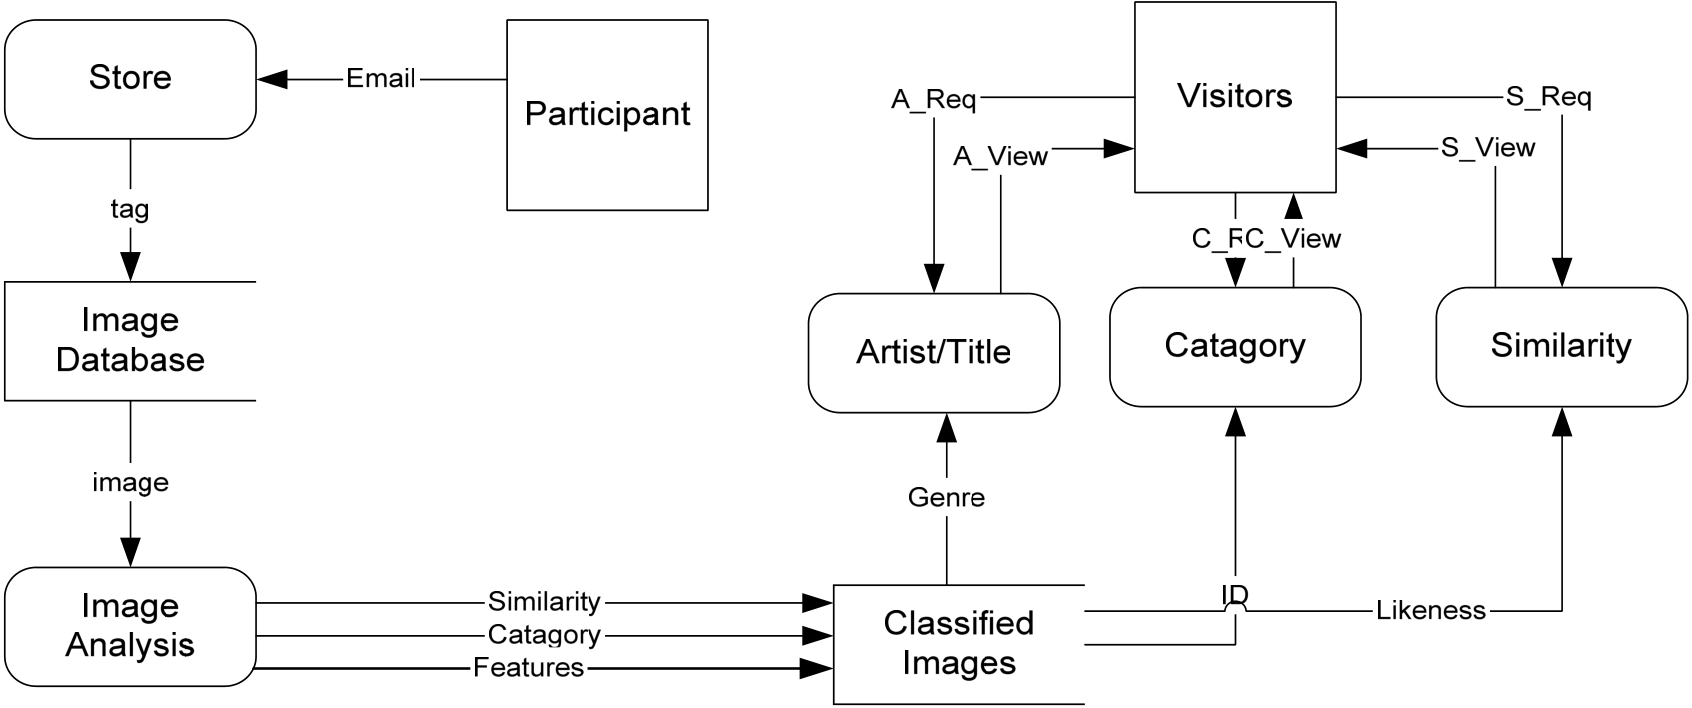
\includegraphics{Fig/media/image69.wmf}

\begin{longtable}[]{@{}
  >{\raggedright\arraybackslash}p{(\columnwidth - 2\tabcolsep) * \real{0.6196}}
  >{\raggedright\arraybackslash}p{(\columnwidth - 2\tabcolsep) * \real{0.3804}}@{}}
\toprule\noalign{}
\begin{minipage}[b]{\linewidth}\raggedright
\textbf{Type}
\end{minipage} & \begin{minipage}[b]{\linewidth}\raggedright

\includegraphics{Fig/media/image84.wmf}
\end{minipage} \\
\midrule\noalign{}
\endhead
\bottomrule\noalign{}
\endlastfoot
All types & 0.18 \\
\end{longtable}

\textbf{Power Rating Factor -} 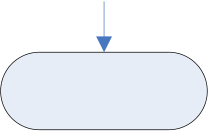
\includegraphics{Fig/media/image75.wmf}


\includegraphics{Fig/media/image85.wmf}

\textbf{Part Quality Factor -} 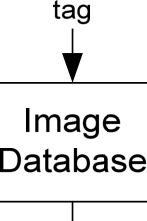
\includegraphics{Fig/media/image79.wmf}

\begin{longtable}[]{@{}
  >{\raggedright\arraybackslash}p{(\columnwidth - 2\tabcolsep) * \real{0.6364}}
  >{\raggedright\arraybackslash}p{(\columnwidth - 2\tabcolsep) * \real{0.3636}}@{}}
\toprule\noalign{}
\begin{minipage}[b]{\linewidth}\raggedright
\textbf{Quality}
\end{minipage} & \begin{minipage}[b]{\linewidth}\raggedright

\includegraphics{Fig/media/image80.wmf}
\end{minipage} \\
\midrule\noalign{}
\endhead
\bottomrule\noalign{}
\endlastfoot
JANTXV & 0.5 \\
JANTX & 1.0 \\
JAN & 2.0 \\
Lower & 5.0 \\
\end{longtable}
\end{minipage} & \begin{minipage}[b]{\linewidth}\raggedright
\end{minipage} & \begin{minipage}[b]{\linewidth}\raggedright
\textbf{Temperature Factor -} 
\includegraphics{Fig/media/image86.wmf}


\includegraphics{Fig/media/image87.wmf}

\textbf{Voltage Stress Factor -} 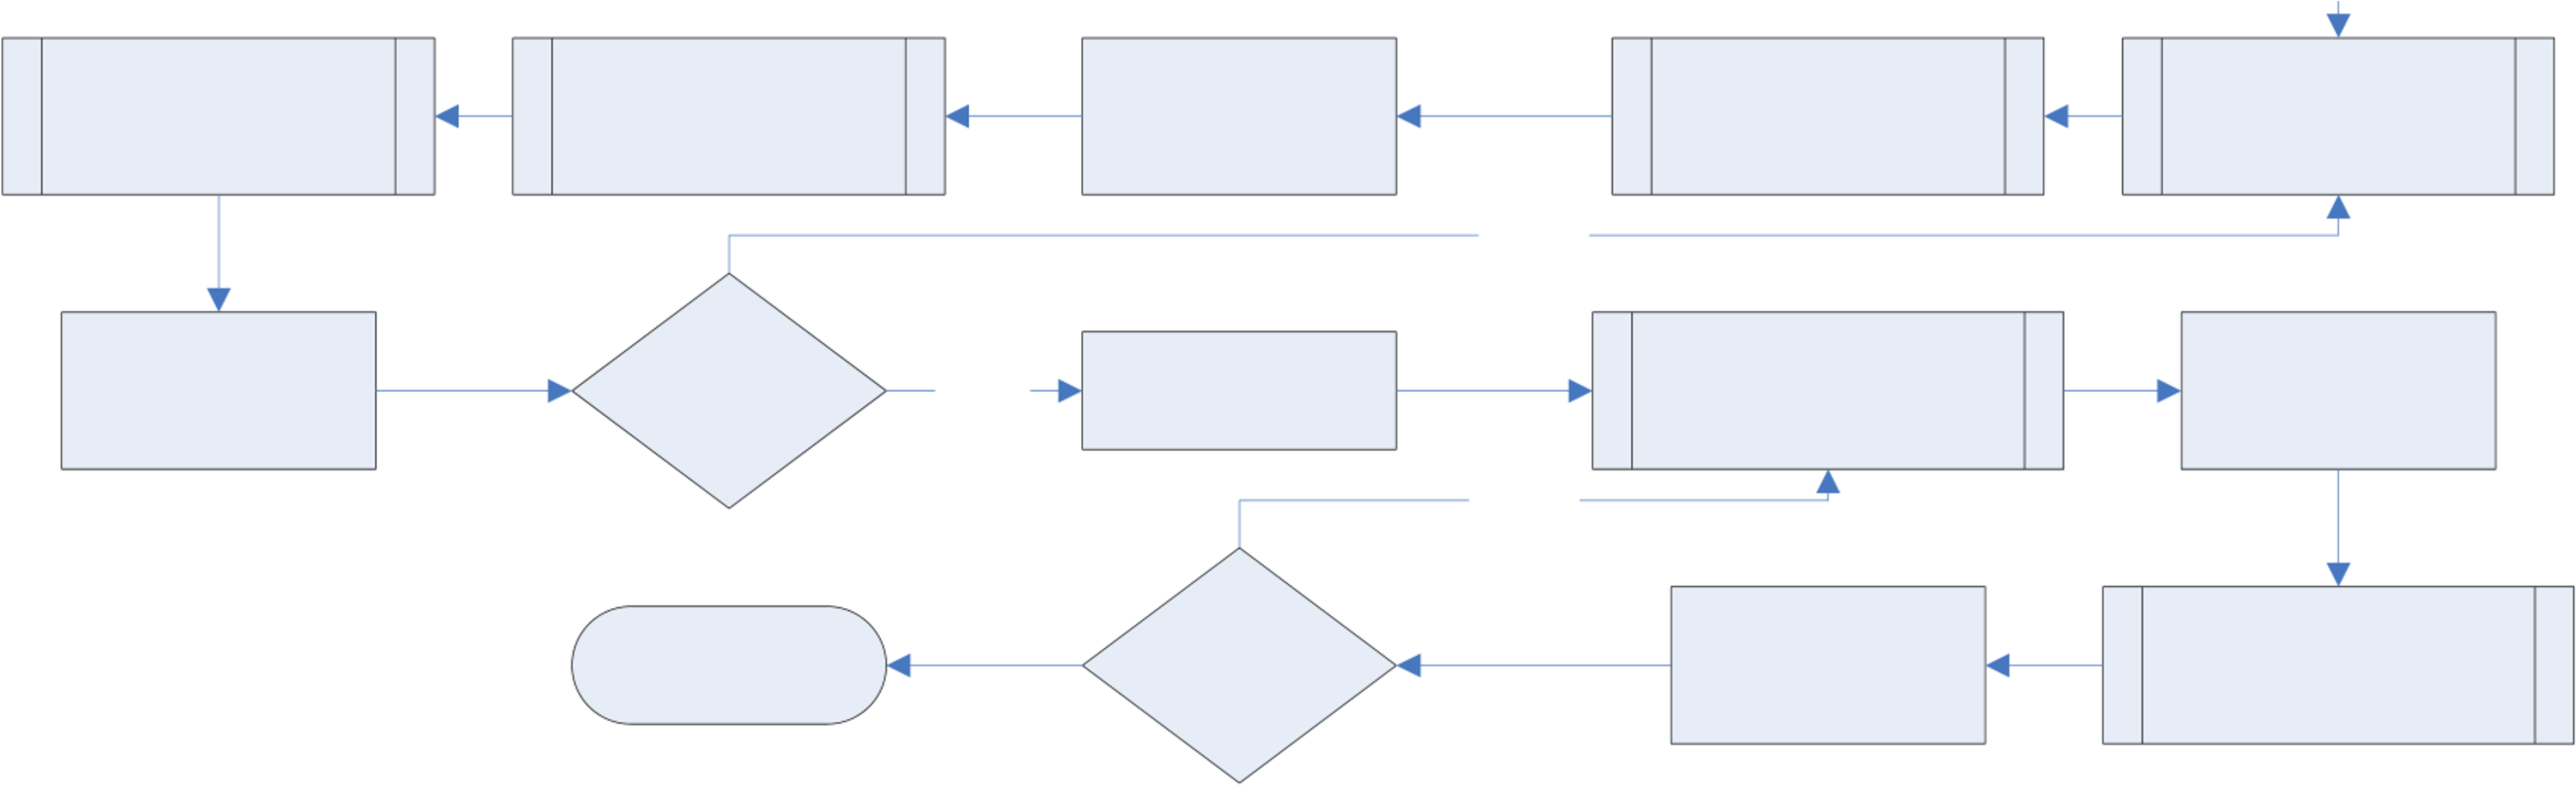
\includegraphics{Fig/media/image77.wmf}


\includegraphics{Fig/media/image88.wmf}

\textbf{Environmental Factor -} 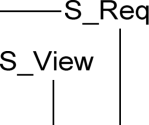
\includegraphics{Fig/media/image89.wmf}

\begin{longtable}[]{@{}
  >{\raggedright\arraybackslash}p{(\columnwidth - 2\tabcolsep) * \real{0.7079}}
  >{\raggedright\arraybackslash}p{(\columnwidth - 2\tabcolsep) * \real{0.2921}}@{}}
\toprule\noalign{}
\begin{minipage}[b]{\linewidth}\raggedright
\textbf{Environment}
\end{minipage} & \begin{minipage}[b]{\linewidth}\raggedright
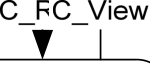
\includegraphics{Fig/media/image90.wmf}
\end{minipage} \\
\midrule\noalign{}
\endhead
\bottomrule\noalign{}
\endlastfoot
G\textsubscript{B} & 1 \\
G\textsubscript{F} & 2 \\
G\textsubscript{M} & 5 \\
N\textsubscript{S} & 4 \\
N\textsubscript{U} & 11 \\
A\textsubscript{IC} & 4 \\
A\textsubscript{IF} & 5 \\
A\textsubscript{UC} & 7 \\
A\textsubscript{UF} & 12 \\
A\textsubscript{RW} & 16 \\
S\textsubscript{F} & 0.50 \\
M\textsubscript{F} & 9 \\
M\textsubscript{L} & 24 \\
C\textsubscript{L} & 250 \\
\end{longtable}
\end{minipage} \\
\midrule\noalign{}
\endhead
\bottomrule\noalign{}
\endlastfoot
\end{longtable}

\subsubsection{\texorpdfstring{\hfill\break
Transistors: Field Effect, Low Frequency (≤
400MHz)}{ Transistors: Field Effect, Low Frequency (≤ 400MHz)}}\label{transistors-field-effect-low-frequency-400mhz}

The failure rate is given by the following relationship

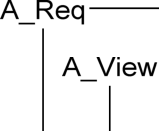
\includegraphics{Fig/media/image91.wmf}.

\begin{longtable}[]{@{}
  >{\raggedright\arraybackslash}p{(\columnwidth - 4\tabcolsep) * \real{0.4619}}
  >{\raggedright\arraybackslash}p{(\columnwidth - 4\tabcolsep) * \real{0.0807}}
  >{\raggedright\arraybackslash}p{(\columnwidth - 4\tabcolsep) * \real{0.4574}}@{}}
\toprule\noalign{}
\begin{minipage}[b]{\linewidth}\raggedright
\textbf{Base Failure Rate -} 
\includegraphics{Fig/media/image92.wmf}

\begin{longtable}[]{@{}
  >{\raggedright\arraybackslash}p{(\columnwidth - 2\tabcolsep) * \real{0.5528}}
  >{\raggedright\arraybackslash}p{(\columnwidth - 2\tabcolsep) * \real{0.4472}}@{}}
\toprule\noalign{}
\begin{minipage}[b]{\linewidth}\raggedright
\textbf{Type}
\end{minipage} & \begin{minipage}[b]{\linewidth}\raggedright
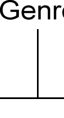
\includegraphics{Fig/media/image93.wmf}
\end{minipage} \\
\midrule\noalign{}
\endhead
\bottomrule\noalign{}
\endlastfoot
MOSFET & 0.012 \\
JFET & 0.0045 \\
\end{longtable}
\end{minipage} & \begin{minipage}[b]{\linewidth}\raggedright
\end{minipage} & \begin{minipage}[b]{\linewidth}\raggedright
\textbf{Temperature Factor -} 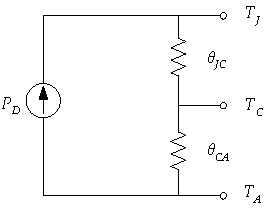
\includegraphics{Fig/media/image94.wmf}

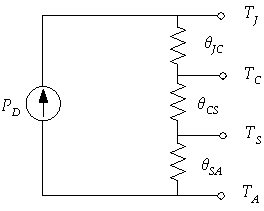
\includegraphics{Fig/media/image95.wmf}
\end{minipage} \\
\midrule\noalign{}
\endhead
\bottomrule\noalign{}
\endlastfoot
\end{longtable}

\begin{longtable}[]{@{}
  >{\raggedright\arraybackslash}p{(\columnwidth - 4\tabcolsep) * \real{0.3743}}
  >{\raggedright\arraybackslash}p{(\columnwidth - 4\tabcolsep) * \real{0.2665}}
  >{\raggedright\arraybackslash}p{(\columnwidth - 4\tabcolsep) * \real{0.3592}}@{}}
\toprule\noalign{}
\begin{minipage}[b]{\linewidth}\raggedright
\textbf{Application Factor -} 
\includegraphics{Fig/media/image96.wmf}

\begin{longtable}[]{@{}
  >{\raggedright\arraybackslash}p{(\columnwidth - 2\tabcolsep) * \real{0.6948}}
  >{\raggedright\arraybackslash}p{(\columnwidth - 2\tabcolsep) * \real{0.3052}}@{}}
\toprule\noalign{}
\begin{minipage}[b]{\linewidth}\raggedright
\textbf{Application (}
\includegraphics{Fig/media/image97.wmf}rated
output power)
\end{minipage} & \begin{minipage}[b]{\linewidth}\raggedright
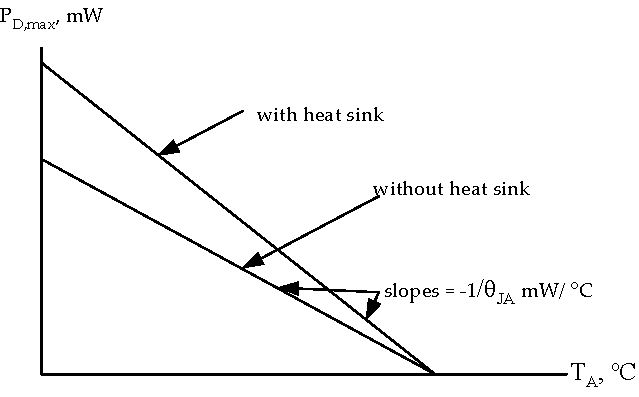
\includegraphics{Fig/media/image98.wmf}
\end{minipage} \\
\midrule\noalign{}
\endhead
\bottomrule\noalign{}
\endlastfoot
Linear Amplification (
\includegraphics{Fig/media/image99.wmf}\textbf{)}

Small Signal

Switching & 1.50

0.70 \\
Power FETs

(Non-linear, 
\includegraphics{Fig/media/image100.wmf}\textbf{)}

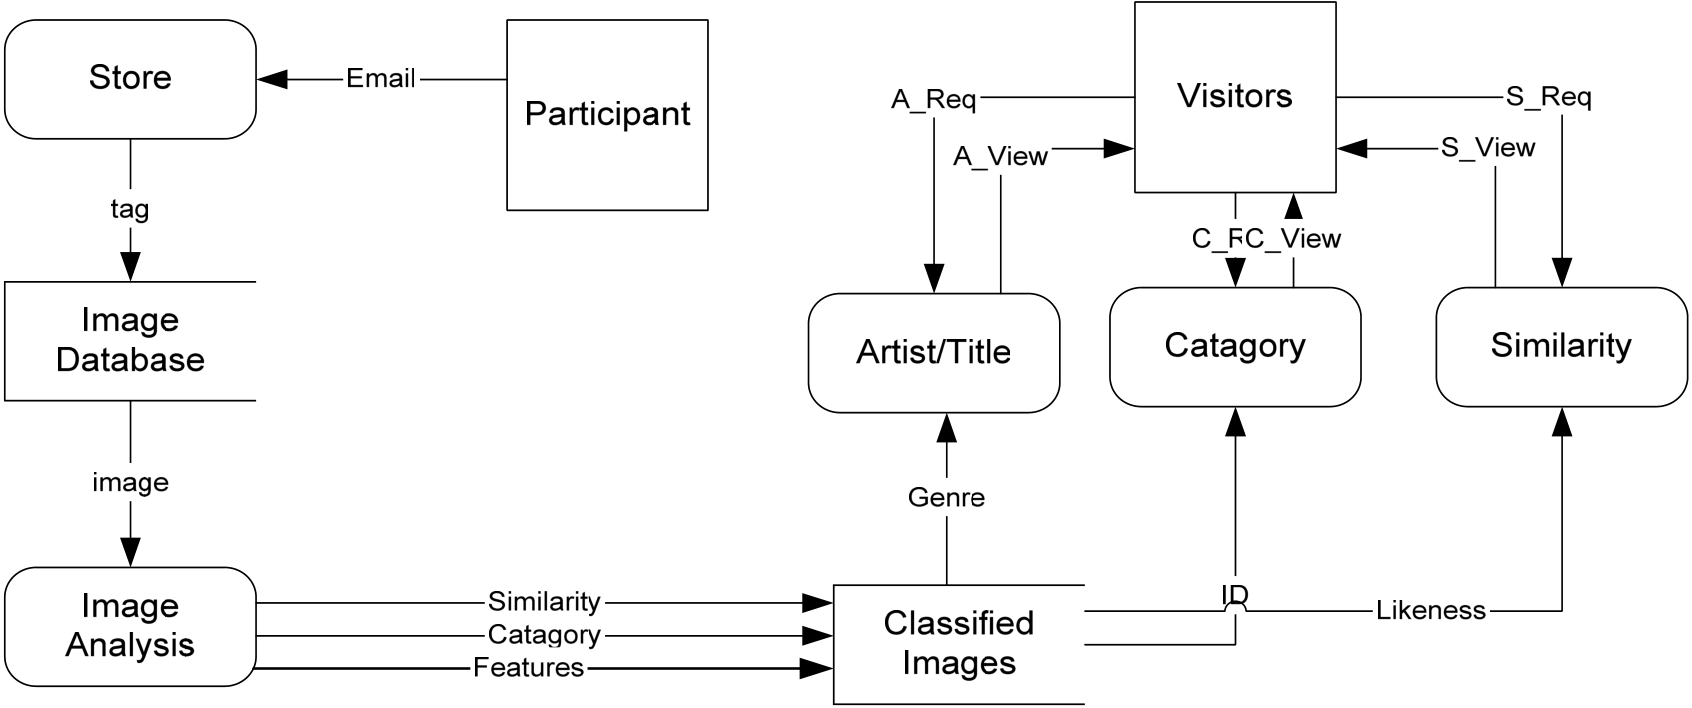
\includegraphics{Fig/media/image101.wmf} &
\includegraphics{Fig/media/image102.wmf} \\
\end{longtable}
\end{minipage} & \begin{minipage}[b]{\linewidth}\raggedright
\textbf{Part Quality Factor -} \includegraphics{Fig/media/image103.wmf}

\begin{longtable}[]{@{}
  >{\raggedright\arraybackslash}p{(\columnwidth - 2\tabcolsep) * \real{0.6539}}
  >{\raggedright\arraybackslash}p{(\columnwidth - 2\tabcolsep) * \real{0.3461}}@{}}
\toprule\noalign{}
\begin{minipage}[b]{\linewidth}\raggedright
\textbf{Quality}
\end{minipage} & \begin{minipage}[b]{\linewidth}\raggedright
\includegraphics{Fig/media/image104.wmf}
\end{minipage} \\
\midrule\noalign{}
\endhead
\bottomrule\noalign{}
\endlastfoot
JANTXV & 0.7 \\
JANTX & 1.0 \\
JAN & 2.4 \\
Lower & 5.5 \\
Plastic & 8.0 \\
\end{longtable}
\end{minipage} & \begin{minipage}[b]{\linewidth}\raggedright
\textbf{Environmental Factor -} \includegraphics{Fig/media/image105.wmf}

\begin{longtable}[]{@{}
  >{\raggedright\arraybackslash}p{(\columnwidth - 2\tabcolsep) * \real{0.7079}}
  >{\raggedright\arraybackslash}p{(\columnwidth - 2\tabcolsep) * \real{0.2921}}@{}}
\toprule\noalign{}
\begin{minipage}[b]{\linewidth}\raggedright
\textbf{Environment}
\end{minipage} & \begin{minipage}[b]{\linewidth}\raggedright
\includegraphics{Fig/media/image106.wmf}
\end{minipage} \\
\midrule\noalign{}
\endhead
\bottomrule\noalign{}
\endlastfoot
G\textsubscript{B} & 1 \\
G\textsubscript{F} & 6 \\
G\textsubscript{M} & 9 \\
N\textsubscript{S} & 9 \\
N\textsubscript{U} & 19 \\
A\textsubscript{IC} & 13 \\
A\textsubscript{IF} & 29 \\
A\textsubscript{UC} & 20 \\
A\textsubscript{UF} & 43 \\
A\textsubscript{RW} & 24 \\
S\textsubscript{F} & 0.50 \\
M\textsubscript{F} & 14 \\
M\textsubscript{L} & 32 \\
C\textsubscript{L} & 320 \\
\end{longtable}
\end{minipage} \\
\midrule\noalign{}
\endhead
\bottomrule\noalign{}
\endlastfoot
\end{longtable}

\subsubsection{\texorpdfstring{\hfill\break
Transistors: Field Effect, High Frequency (\textgreater{} 400MHz), Low
Power (≤
300mW)}{ Transistors: Field Effect, High Frequency (\textgreater{} 400MHz), Low Power (≤ 300mW)}}\label{transistors-field-effect-high-frequency-400mhz-low-power-300mw}

The failure rate is given by the following relationship

\includegraphics{Fig/media/image107.wmf}.

\begin{longtable}[]{@{}
  >{\raggedright\arraybackslash}p{(\columnwidth - 4\tabcolsep) * \real{0.4619}}
  >{\raggedright\arraybackslash}p{(\columnwidth - 4\tabcolsep) * \real{0.0807}}
  >{\raggedright\arraybackslash}p{(\columnwidth - 4\tabcolsep) * \real{0.4574}}@{}}
\toprule\noalign{}
\begin{minipage}[b]{\linewidth}\raggedright
\textbf{Base Failure Rate -} \includegraphics{Fig/media/image108.wmf}

\begin{longtable}[]{@{}
  >{\raggedright\arraybackslash}p{(\columnwidth - 2\tabcolsep) * \real{0.7071}}
  >{\raggedright\arraybackslash}p{(\columnwidth - 2\tabcolsep) * \real{0.2929}}@{}}
\toprule\noalign{}
\begin{minipage}[b]{\linewidth}\raggedright
\textbf{Type}
\end{minipage} & \begin{minipage}[b]{\linewidth}\raggedright
\includegraphics{Fig/media/image109.wmf}
\end{minipage} \\
\midrule\noalign{}
\endhead
\bottomrule\noalign{}
\endlastfoot
MOSFET & 0.060 \\
JFET & 0.023 \\
\end{longtable}

\textbf{Temperature Factor -} \includegraphics{Fig/media/image110.wmf}

\includegraphics{Fig/media/image111.wmf}
\end{minipage} & \begin{minipage}[b]{\linewidth}\raggedright
\end{minipage} & \begin{minipage}[b]{\linewidth}\raggedright
\textbf{Part Quality Factor -} \includegraphics{Fig/media/image112.wmf}

\begin{longtable}[]{@{}
  >{\raggedright\arraybackslash}p{(\columnwidth - 2\tabcolsep) * \real{0.6488}}
  >{\raggedright\arraybackslash}p{(\columnwidth - 2\tabcolsep) * \real{0.3512}}@{}}
\toprule\noalign{}
\begin{minipage}[b]{\linewidth}\raggedright
\textbf{Quality}
\end{minipage} & \begin{minipage}[b]{\linewidth}\raggedright
\includegraphics{Fig/media/image113.wmf}
\end{minipage} \\
\midrule\noalign{}
\endhead
\bottomrule\noalign{}
\endlastfoot
JANTXV & 0.5 \\
JANTX & 1.0 \\
JAN & 2.0 \\
Lower & 5.0 \\
\end{longtable}
\end{minipage} \\
\midrule\noalign{}
\endhead
\bottomrule\noalign{}
\endlastfoot
\end{longtable}

\textbf{Environmental Factor -} \includegraphics{Fig/media/image114.wmf}

\begin{longtable}[]{@{}
  >{\raggedright\arraybackslash}p{(\columnwidth - 2\tabcolsep) * \real{0.7079}}
  >{\raggedright\arraybackslash}p{(\columnwidth - 2\tabcolsep) * \real{0.2921}}@{}}
\toprule\noalign{}
\begin{minipage}[b]{\linewidth}\raggedright
\textbf{Environment}
\end{minipage} & \begin{minipage}[b]{\linewidth}\raggedright
\includegraphics{Fig/media/image115.wmf}
\end{minipage} \\
\midrule\noalign{}
\endhead
\bottomrule\noalign{}
\endlastfoot
G\textsubscript{B} & 1 \\
G\textsubscript{F} & 2 \\
G\textsubscript{M} & 5 \\
N\textsubscript{S} & 4 \\
N\textsubscript{U} & 11 \\
A\textsubscript{IC} & 4 \\
A\textsubscript{IF} & 5 \\
A\textsubscript{UC} & 7 \\
A\textsubscript{UF} & 12 \\
A\textsubscript{RW} & 16 \\
S\textsubscript{F} & 0.50 \\
M\textsubscript{F} & 9 \\
M\textsubscript{L} & 24 \\
C\textsubscript{L} & 250 \\
\end{longtable}

\subsubsection{Microcircuits: Gate/Logic Arrays and
Microprocessors}\label{microcircuits-gatelogic-arrays-and-microprocessors}

Includes the following devices:

\begin{enumerate}
\def\labelenumi{\arabic{enumi}.}
\item
  Bipolar devices, Digital and Linear Gate/Logic Arrays
\item
  MOS Devices, Digital and Linear Gate/Logic Arrays
\item
  Field Programmable Logic Array (PLA) and Programmable Array Logic
  (PAL)
\item
  Microprocessors
\end{enumerate}

The failure rate is given by the following relationship

\includegraphics{Fig/media/image116.wmf} .

\includegraphics{Fig/media/image117.wmf} = \textbf{Complexity Failure
Rate for Bipolar Devices (Digital and Linear Gate/Logic)}

\begin{longtable}[]{@{}
  >{\raggedright\arraybackslash}p{(\columnwidth - 10\tabcolsep) * \real{0.2212}}
  >{\raggedright\arraybackslash}p{(\columnwidth - 10\tabcolsep) * \real{0.1152}}
  >{\raggedright\arraybackslash}p{(\columnwidth - 10\tabcolsep) * \real{0.1935}}
  >{\raggedright\arraybackslash}p{(\columnwidth - 10\tabcolsep) * \real{0.1106}}
  >{\raggedright\arraybackslash}p{(\columnwidth - 10\tabcolsep) * \real{0.1843}}
  >{\raggedright\arraybackslash}p{(\columnwidth - 10\tabcolsep) * \real{0.1751}}@{}}
\toprule\noalign{}
\multicolumn{2}{@{}>{\raggedright\arraybackslash}p{(\columnwidth - 10\tabcolsep) * \real{0.3364} + 2\tabcolsep}}{%
\begin{minipage}[b]{\linewidth}\raggedright
\textbf{Digital}
\end{minipage}} &
\multicolumn{2}{>{\raggedright\arraybackslash}p{(\columnwidth - 10\tabcolsep) * \real{0.3041} + 2\tabcolsep}}{%
\begin{minipage}[b]{\linewidth}\raggedright
\textbf{Linear}
\end{minipage}} &
\multicolumn{2}{>{\raggedright\arraybackslash}p{(\columnwidth - 10\tabcolsep) * \real{0.3594} + 2\tabcolsep}@{}}{%
\begin{minipage}[b]{\linewidth}\raggedright
\textbf{PLA/PAL}
\end{minipage}} \\
\midrule\noalign{}
\endhead
\bottomrule\noalign{}
\endlastfoot
No. Gates & \includegraphics{Fig/media/image118.wmf} & No. Transistors &
\includegraphics{Fig/media/image119.wmf} & No. Gates &
\includegraphics{Fig/media/image120.wmf} \\
1 to 100

101 to 1,000

1,001 to 3,000

3,001 to 10,000

10,001 to 30,000

30,001 to 60,000 & 0.0025

0.0050

0.010

0.020

0.040

0.080 & 1 to 100

101 to 300

301 to 1,000

1,001 to 10,000 & 0.010

0.020

0.040

0.060 & Up to 200

201 to 1,000

1,001 to 5,000 & 0.010

0.021

0.042 \\
\end{longtable}

\includegraphics{Fig/media/image121.wmf} = \textbf{Complexity Failure
Rate for MOS Devices (Digital and Linear Gate/Logic)}

\begin{longtable}[]{@{}
  >{\raggedright\arraybackslash}p{(\columnwidth - 10\tabcolsep) * \real{0.2192}}
  >{\raggedright\arraybackslash}p{(\columnwidth - 10\tabcolsep) * \real{0.1142}}
  >{\raggedright\arraybackslash}p{(\columnwidth - 10\tabcolsep) * \real{0.1918}}
  >{\raggedright\arraybackslash}p{(\columnwidth - 10\tabcolsep) * \real{0.1096}}
  >{\raggedright\arraybackslash}p{(\columnwidth - 10\tabcolsep) * \real{0.1826}}
  >{\raggedright\arraybackslash}p{(\columnwidth - 10\tabcolsep) * \real{0.1826}}@{}}
\toprule\noalign{}
\multicolumn{2}{@{}>{\raggedright\arraybackslash}p{(\columnwidth - 10\tabcolsep) * \real{0.3333} + 2\tabcolsep}}{%
\begin{minipage}[b]{\linewidth}\raggedright
\textbf{Digital}
\end{minipage}} &
\multicolumn{2}{>{\raggedright\arraybackslash}p{(\columnwidth - 10\tabcolsep) * \real{0.3014} + 2\tabcolsep}}{%
\begin{minipage}[b]{\linewidth}\raggedright
\textbf{Linear}
\end{minipage}} &
\multicolumn{2}{>{\raggedright\arraybackslash}p{(\columnwidth - 10\tabcolsep) * \real{0.3653} + 2\tabcolsep}@{}}{%
\begin{minipage}[b]{\linewidth}\raggedright
\textbf{MOS}
\end{minipage}} \\
\midrule\noalign{}
\endhead
\bottomrule\noalign{}
\endlastfoot
No. Gates & \includegraphics{Fig/media/image122.wmf} & No. Transistors &
\includegraphics{Fig/media/image122.wmf} & No. Gates &
\includegraphics{Fig/media/image122.wmf} \\
1 to 100

101 to 1,000

1,001 to 3,000

3,001 to 10,000

10,001 to 30,000

30,001 to 60,000 & 0.010

0.020

0.040

0.080

0.16

0.29 & 1 to 100

101 to 300

301 to 1,000

1,001 to 10,000 & 0.010

0.020

0.040

0.060 & Up to 500

501 to 1,000

1,001 to 5,000

5,001 to 20,000 & 0.00085

0.0017

0.0034

0.0068 \\
\end{longtable}

\includegraphics{Fig/media/image123.wmf} = \textbf{Complexity Failure
Rate for Microprocessors}

\begin{longtable}[]{@{}
  >{\raggedright\arraybackslash}p{(\columnwidth - 4\tabcolsep) * \real{0.3354}}
  >{\raggedright\arraybackslash}p{(\columnwidth - 4\tabcolsep) * \real{0.3165}}
  >{\raggedright\arraybackslash}p{(\columnwidth - 4\tabcolsep) * \real{0.3481}}@{}}
\toprule\noalign{}
\begin{minipage}[b]{\linewidth}\raggedright
\textbf{Number of Bits}
\end{minipage} & \begin{minipage}[b]{\linewidth}\raggedright
\includegraphics{Fig/media/image123.wmf} \textbf{- Bipolar}
\end{minipage} & \begin{minipage}[b]{\linewidth}\raggedright
\includegraphics{Fig/media/image123.wmf} \textbf{- MOS}
\end{minipage} \\
\midrule\noalign{}
\endhead
\bottomrule\noalign{}
\endlastfoot
Up to 8

Up to 16

Up to 32 & 0.060

0.12

0.24 & 0.14

0.28

0.56 \\
\end{longtable}

\includegraphics{Fig/media/image124.wmf} = \textbf{Package Failure Rate
for all microcircuits.} \includegraphics{Fig/media/image125.wmf}
\textbf{= number of pins on package.}

\includegraphics{Fig/media/image126.wmf}

\textbf{Temperature Factor -} \includegraphics{Fig/media/image127.wmf}

\includegraphics{Fig/media/image128.wmf}

The activation energy (\includegraphics{Fig/media/image129.wmf}) for
different technologies are given in the table below.

\begin{longtable}[]{@{}
  >{\raggedright\arraybackslash}p{(\columnwidth - 12\tabcolsep) * \real{0.1461}}
  >{\raggedright\arraybackslash}p{(\columnwidth - 12\tabcolsep) * \real{0.1545}}
  >{\raggedright\arraybackslash}p{(\columnwidth - 12\tabcolsep) * \real{0.1385}}
  >{\raggedright\arraybackslash}p{(\columnwidth - 12\tabcolsep) * \real{0.1392}}
  >{\raggedright\arraybackslash}p{(\columnwidth - 12\tabcolsep) * \real{0.1295}}
  >{\raggedright\arraybackslash}p{(\columnwidth - 12\tabcolsep) * \real{0.1497}}
  >{\raggedright\arraybackslash}p{(\columnwidth - 12\tabcolsep) * \real{0.1425}}@{}}
\toprule\noalign{}
\begin{minipage}[b]{\linewidth}\raggedright
\textbf{Technology}
\end{minipage} & \begin{minipage}[b]{\linewidth}\raggedright
\textbf{TTL, ASTLL, CML, HTTL, FTLL, DTL, ECL, ALSTTL}
\end{minipage} & \begin{minipage}[b]{\linewidth}\raggedright
\textbf{F, LTTL, STTL}
\end{minipage} & \begin{minipage}[b]{\linewidth}\raggedright
\textbf{BiCMOS LSTTL}
\end{minipage} & \begin{minipage}[b]{\linewidth}\raggedright
\textbf{Digital MOS, VHSIC CMOS}
\end{minipage} & \begin{minipage}[b]{\linewidth}\raggedright
\textbf{Linear (Bipolar and MOS)}
\end{minipage} & \begin{minipage}[b]{\linewidth}\raggedright
\textbf{Memories (Bipolar and MOS), NMOS}
\end{minipage} \\
\midrule\noalign{}
\endhead
\bottomrule\noalign{}
\endlastfoot
\includegraphics{Fig/media/image130.wmf} & 0.4 & 0.45 & 0.5 & 0.35 &
0.65 & 0.6 \\
\end{longtable}

\begin{longtable}[]{@{}
  >{\raggedright\arraybackslash}p{(\columnwidth - 4\tabcolsep) * \real{0.4619}}
  >{\raggedright\arraybackslash}p{(\columnwidth - 4\tabcolsep) * \real{0.0807}}
  >{\raggedright\arraybackslash}p{(\columnwidth - 4\tabcolsep) * \real{0.4574}}@{}}
\toprule\noalign{}
\begin{minipage}[b]{\linewidth}\raggedright
\textbf{Learning Factor -} \includegraphics{Fig/media/image131.wmf}

\begin{longtable}[]{@{}
  >{\raggedright\arraybackslash}p{(\columnwidth - 2\tabcolsep) * \real{0.6944}}
  >{\raggedright\arraybackslash}p{(\columnwidth - 2\tabcolsep) * \real{0.3056}}@{}}
\toprule\noalign{}
\begin{minipage}[b]{\linewidth}\raggedright
\textbf{Years in Production}
\end{minipage} & \begin{minipage}[b]{\linewidth}\raggedright
\includegraphics{Fig/media/image132.wmf}
\end{minipage} \\
\midrule\noalign{}
\endhead
\bottomrule\noalign{}
\endlastfoot
\includegraphics{Fig/media/image133.wmf}.1 & 2.0 \\
0.5 & 1.8 \\
1.0 & 1.5 \\
1.5 & 1.2 \\
\includegraphics{Fig/media/image134.wmf} & 1.0 \\
\end{longtable}
\end{minipage} & \begin{minipage}[b]{\linewidth}\raggedright
\end{minipage} & \begin{minipage}[b]{\linewidth}\raggedright
\textbf{Part Quality Factor -} \includegraphics{Fig/media/image135.wmf}

\begin{longtable}[]{@{}
  >{\raggedright\arraybackslash}p{(\columnwidth - 2\tabcolsep) * \real{0.6050}}
  >{\raggedright\arraybackslash}p{(\columnwidth - 2\tabcolsep) * \real{0.3950}}@{}}
\toprule\noalign{}
\begin{minipage}[b]{\linewidth}\raggedright
\textbf{Quality}
\end{minipage} & \begin{minipage}[b]{\linewidth}\raggedright
\includegraphics{Fig/media/image136.wmf}
\end{minipage} \\
\midrule\noalign{}
\endhead
\bottomrule\noalign{}
\endlastfoot
S & 0.25 \\
B & 1.0 \\
B-1 & 2.0 \\
\end{longtable}
\end{minipage} \\
\midrule\noalign{}
\endhead
\bottomrule\noalign{}
\endlastfoot
\end{longtable}

\textbf{Environmental Factor -} \includegraphics{Fig/media/image137.wmf}

\begin{longtable}[]{@{}
  >{\raggedright\arraybackslash}p{(\columnwidth - 2\tabcolsep) * \real{0.7079}}
  >{\raggedright\arraybackslash}p{(\columnwidth - 2\tabcolsep) * \real{0.2921}}@{}}
\toprule\noalign{}
\begin{minipage}[b]{\linewidth}\raggedright
\textbf{Environment}
\end{minipage} & \begin{minipage}[b]{\linewidth}\raggedright
\includegraphics{Fig/media/image138.wmf}
\end{minipage} \\
\midrule\noalign{}
\endhead
\bottomrule\noalign{}
\endlastfoot
G\textsubscript{B} & 0.50 \\
G\textsubscript{F} & 2 \\
G\textsubscript{M} & 4 \\
N\textsubscript{S} & 4 \\
N\textsubscript{U} & 6 \\
A\textsubscript{IC} & 4 \\
A\textsubscript{IF} & 5 \\
A\textsubscript{UC} & 5 \\
A\textsubscript{UF} & 8 \\
A\textsubscript{RW} & 8 \\
S\textsubscript{F} & 0.50 \\
M\textsubscript{F} & 5 \\
M\textsubscript{L} & 12 \\
C\textsubscript{L} & 220 \\
\end{longtable}
